\subsection{Existence of diffusion speed heterogeneity}
We make an interesting analysis of message's diffusion speed on 2 real world datasets: Sina microblog and U.S. patent. We normalize the activation times with Min-Max method and divide the time length of cascade into several periods.
As diffusion speed is unmeasurable, we compute the $\frac{1}{\overline{\Delta t}}$ in each life span that is proportion to the ground truth diffusion speed. As in Figure \ref{fig:PatentHetero}, the maximum of $\frac{1}{\overline{\Delta t}}$ reaches 80 in Sina and about 12 in Patent dataset, while the minimum approaches 0. There is distinct difference of diffusion speed in different life span. However, former algorithms have not taken this into consideration. They assume that the coefficient of $\Delta t$'s distribution which controls diffusion speed does not change with time. We believe the life span heterogeneity is a key point to re-understand network inference problem.
\begin{figure}[H]
\subfigure[Cascades of Sina Microblog dataset]{\centerline{
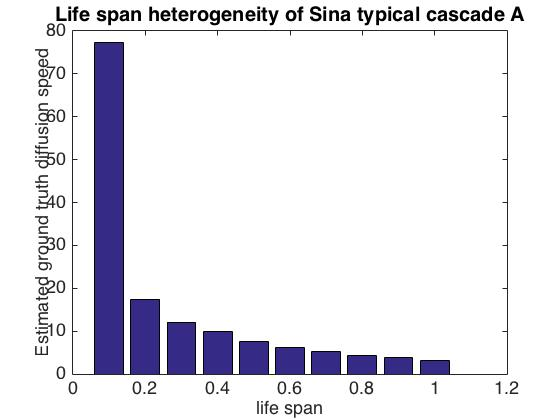
\includegraphics[width=0.55\linewidth]{figures/SinaA.jpg}
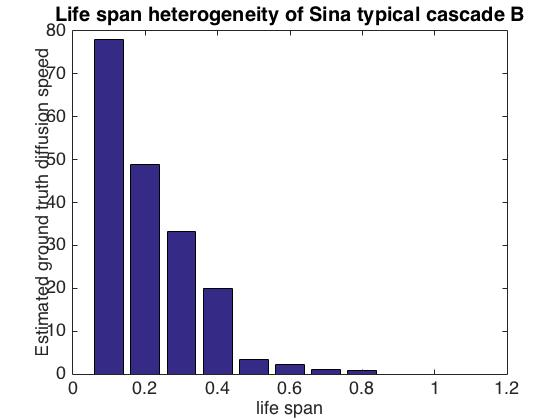
\includegraphics[width=0.55\linewidth]{figures/SinaB.jpg}}}
\subfigure[Cascades of U.S. Patent dataset]{\centerline{
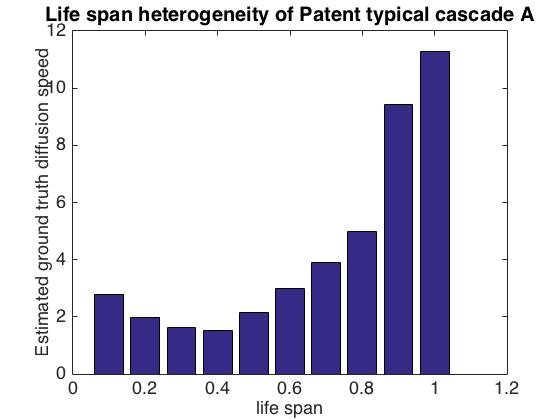
\includegraphics[width=0.55\linewidth]{figures/PatentA.jpg}
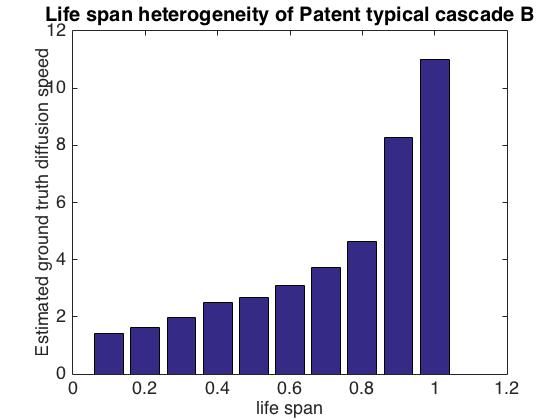
\includegraphics[width=0.55\linewidth]{figures/PatentB.jpg}}}
\caption{The diffusion speed of 2 real world dataset differs a lot in different life span. }\label{fig:PatentHetero}
\end{figure}
%==========================
\subsection{Validity of diffusion speed approximation approach}
We aim to make use of diffusion speed information in network inference algorithm. But the estimation of diffusion speed requires the parent relationship in cascades which is seldom available in real world data, we would like to use the number of activated nodes as surrogate for the diffusion speed, which is:
\begin{equation}
S_p(t_j)=(I^{t_j+lag}-I^{t_j-lag})/I^T
\end{equation}
$t_j$ is the target time stamp. $lag$ is half the length of sliding window around $t_j$, $T$ is the end of every cascade. $I^t$ refers to the number of infected nodes by time $t$. The value of $S_p(t_j)$ ranges from 0 to 1.
\\We show the validity of this approach by empirically calculating the correlation. We select 80 long cascades in Patent dataset and 50 long cascades in Sina dataset. As in Table \ref{tab:Corre}, we use Evans's (1996) interpretation for r coefficient to describe the strength of correlation. 65\% of Patent cascades and 90\% of Sina cascades present strong or very stronger correlation. Our approach of calculating activated nodes number can reflect the level of diffusion speed to a large extent.
\begin{table}[H]
\caption{Correlation coefficients between ground truth diffusion speed and the number of activated nodes in time unit.}
\begin{tabular}{c|c|c|c}
 coefficient range & strength & pct. Patent & pct. Sina \\
\hline
.00-.19 & very weak & 0.05 & 0.02\\
.20-.39 & weak & 0.125 & 0.02\\
.40-.59 & moderate & 0.175 & 0.06\\
.60-.79 & strong & 0.3 & 0.08\\
.80-1.0 & very strong & 0.35 & 0.82\\
\end{tabular}\label{tab:Corre}
\end{table}